\documentclass{beamer}
\mode<presentation>

\usetheme{Frankfurt}
\usecolortheme{beaver}

\setbeamertemplate{navigation symbols}{}
\setbeamersize{text margin left=2.5ex,text margin right=2.5ex}

\definecolor{DarkRed}{RGB}{178,16,49}
\definecolor{Gold}{RGB}{227,174,9}

\setbeamercolor*{title}{use=structure,fg=white,bg=DarkRed!80}
\setbeamercolor{frametitle}{use=structure,fg=DarkRed,bg=lightgray!20}
\setbeamertemplate{title page}[default][colsep=-4bp,rounded=true,shadow=true]

\setbeamercolor{block title}{use=structure,fg=white,bg=DarkRed!85}
\setbeamercolor{block body}{parent=normal text,use=block title,bg=black!5}

\setbeamercolor{item}{fg=DarkRed}

\setbeamercolor{section in head/foot}{bg=lightgray!50,fg=DarkRed}
\setbeamercolor{title in head/foot}{bg=lightgray!20,fg=DarkRed}
\setbeamercolor{date in head/foot}{bg=lightgray!60,fg=DarkRed}
%\setbeamercolor{subsection in head/foot}{bg=gray!30,fg=black}

\makeatletter
\setbeamertemplate{footline}
{
	\leavevmode
	\hbox{%
		\begin{beamercolorbox}[wd=.33333333333\paperwidth,ht=2.25ex,dp=1ex,center]{title}
			\usebeamerfont{author in head/foot}\insertshortauthor~~\beamer@ifempty{\insertshortinstitute}{}{(\insertshortinstitute)}
		\end{beamercolorbox}%
		\begin{beamercolorbox}[wd=.33333333333\paperwidth,ht=2.25ex,dp=1ex,center]{title in head/foot}
			\usebeamerfont{title in head/foot}\insertshorttitle
		\end{beamercolorbox}%
		\begin{beamercolorbox}[wd=.33333333333\paperwidth,ht=2.25ex,dp=1ex,right]{date in head/foot}
			\usebeamerfont{date in head/foot}\hspace*{2em}
			\insertshortdate{}\hspace*{4em}
			\insertframenumber{} / \inserttotalframenumber\hspace*{3ex} 
		\end{beamercolorbox}
	}
	\vskip0pt
}

\newcommand{\emptyheadline}{
	\setbeamertemplate{headline}
	{
		\leavevmode
		\hbox{%
			\begin{beamercolorbox}[wd=.5\paperwidth,ht=2.25ex,dp=1.125ex,left]{title}
			\end{beamercolorbox}%
			\begin{beamercolorbox}[wd=.5\paperwidth,ht=2.25ex,dp=1.125ex,right]{section in head/foot}
			\end{beamercolorbox}%
			\begin{beamercolorbox}[wd=.05\paperwidth,ht=2.25ex,dp=5ex,right]{section in head/foot}
			\end{beamercolorbox}
		}
		\vskip0pt
	}
}
\makeatother

\newcommand{\corresponding}[1]{\textcolor{DarkRed}{\emph{#1}}}

\newcommand{\tcite}[1]{\textsuperscript{\textcolor{Gold}{\tiny\cite{#1}}}}

\newcommand{\eg}{\item[e.g.]}
\newcommand{\ie}{\item[i.e.]}
\newcommand{\wip}{\item[w.i.p.]}
\newcommand{\arrow}{\item[$\rightarrow$]}
\newcommand{\yes}{\item[\ding{51}]}
\newcommand{\no}{\item[\ding{56}]}
\newcommand{\lookat}{\item[\ding{43}]}

\usepackage{SC-AITA-2023}
\usepackage{pifont}
\usepackage{subfig}
\usepackage{booktabs}
\newcommand\fourinarow{0.235\linewidth}
\newcommand{\creepy}{\textsc{CReEPy}}
\newcommand{\exact}{\textsc{ExACT}}

\usepackage{listings}
\lstset{%
	backgroundcolor=\color{white},
	basicstyle={\scriptsize\ttfamily},% footnotesize acceptable for monospace
	numbers=left,numberstyle=\footnotesize,xleftmargin=2em,% show line numbers, remove this entire line if you don't want the numbers.
	breakatwhitespace=false,
	frame=single,
	language=Prolog,
	numbers=left,
	numbersep=5pt,
	numberstyle=\tiny\color{gray},
	keywordstyle=\color{black},
	showstringspaces=false,tabsize=2,breaklines=true}

\title[Evaluation of Symbolic Knowledge]
{On the Evaluation of the Symbolic Knowledge Extracted from Black Boxes}
%
\author[F. Sabbatini, R. Calegari]{
	\vspace{-2ex} \\
	{Federico Sabbatini$^*$} % empth the presenting author
	\and
	\corresponding{Roberta Calegari$^\dagger$}
}
\vspace{-0.5cm}
\institute[UniBo]{
	$^*$Department of Pure and Applied Sciences (DiSPeA) -- University of Urbino
	\\
	$^\dagger$Alma Mater Research Institute for Human-Centered Artificial Intelligence -- \textsc{Alma Mater Studiorum}---University of Bologna
	\\ \smallskip
	{f.sabbatini@unibo.it},
	\corresponding{roberta.calegari@unibo.it}
}

\date[AITA, 2023]{\small AAAI Spring Symposium 2023 -- AITA: AI Trustworthiness Assessment\\March 27--29, 2023, San Francisco, California, USA}

\AtBeginSection[]
{
	\begin{frame}<beamer>[c,noframenumbering]
		\frametitle{Next in Line\ldots}
		\tableofcontents[sectionstyle=show/shaded,subsectionstyle=hide]
	\end{frame}
}

\AtBeginSubsection[]
{
	\begin{frame}<beamer>[shrink,noframenumbering]
		\frametitle{Focus on\ldots}
		\mbox{~}
		\tableofcontents[currentsubsection,sectionstyle=shaded,subsectionstyle=show/shaded]
		\mbox{~}
	\end{frame}
}
\titlegraphic{
{{
\includegraphics[width=0.15\textwidth]{img/tailor-logo.png}
\tiny This work has been partially supported by the EU ICT-48 2020 project TAILOR (No. 952215).}}
}

\begin{document}
	\begingroup
		\emptyheadline
		\frame{\titlepage}
	\endgroup

\section{Context \& Motivation}

\begin{frame}[c]{Context}
	\begin{block}{Black-box predictors}
	
		\begin{itemize}
			\item currently adopted in almost every field~\tcite{rocha2012far}
			\begin{itemize}
				\eg pattern detection, image and speech recognition
			\end{itemize}
			\item detect patterns and relationships buried in data
			
			\smallskip 
			
			\yes knowledge acquired and reused in similar applications
			\begin{itemize}
				\yes impressive predictive capabilities
			\end{itemize}
		
			\smallskip
			
			\no knowledge sub-symbolically represented (internal parameters)
			\begin{itemize}
				\no internal logic \alert{hidden} to users
				\no not suitable for human comprehension (BB behaviour~\tcite{Lipton2018})
				\no no \alert{explanations} provided for predictions
			\end{itemize}
		
			\smallskip

			\arrow unreliability in critical applications
			\begin{itemize}
				\eg healthcare, finance, etc.
			\end{itemize}
	
			\smallskip
			
			\lookat interpretable predictors, \alert{symbolic knowledge-extraction techniques}
		\end{itemize}
	\end{block}
\end{frame}

\begin{frame}[c]{Motivation}
	
	\begin{block}{SKE techniques}
		\medskip
		More and more different extraction techniques are available, however:
		\begin{itemize}
			\item corresponding outputs should be ``manually'' compared
			\medskip
			\lookat \alert{advantages in exploiting autoML techniques}, but
			\no no suitable metrics to evaluate the available alternatives	
			\medskip
			\item there is not a unique knowledge representation
			\begin{itemize}
				\no comparison between knowledge from different SKE techniques
			\end{itemize}
			\medskip
			\item there is not a unique rule representation
			\begin{itemize}
				\no difficult comparison between rules of different KB
			\end{itemize}
		\end{itemize}
		\medskip
	\end{block}
\end{frame}

\begin{frame}[c,allowframebreaks]{Contribution}
	\vfill
	\begin{block}{Discussing major issues about knowledge readability metrics}
		\medskip
		\begin{itemize}
			\item Depth of readability
			\begin{itemize}
				\item considering the knowledge as a whole
				\item considering individual rules
			\end{itemize}
			\medskip
			\lookat Levels of readability
			\begin{itemize}
				\item macrolevel
				\begin{itemize}
					\eg shape of the knowledge
					\eg size of the knowledge
				\end{itemize}
				\item microlevel
				\begin{itemize}
					\eg shape of the rules
					\eg complexity of the rules
				\end{itemize}
			\end{itemize}
		\end{itemize}
		\medskip
	\end{block}
	\vfill
	
	\framebreak
	
	\vfill 
	
	\begin{block}{Formulating a scoring function evaluating the knowledge quality}
		\medskip
		\begin{itemize}
			\item Several indices affecting the knowledge quality
			\begin{itemize}
				\eg predictive performance
				\eg readability
				\eg completeness
			\end{itemize}
			\medskip
			\item Need of a compact scoring function
			\medskip
			\lookat Novel metric to assess the knowledge quality
			\begin{itemize}
				\item encompassing several relevant quality indices
			\end{itemize}
		\end{itemize}
		\medskip
	\end{block}
\end{frame}

%\section{Evaluating Knowledge Extracted via SKE}
\section{On Quality Evaluation}

\begin{frame}[c]{Knowledge Quality Evaluation}
	\vfill
	\begin{block}{Common evaluation metrics~\tcite{garcez2001symbolic,tran2013knowledge}}
		\medskip
		\begin{itemize}
			\item Predictive performance, task-dependent
			\begin{itemize}
				\eg w.r.t.\ the data
				\eg w.r.t.\ the underlying BB (\emph{fidelity})
			\end{itemize}
			\medskip
			\item Input space coverage (\emph{completeness})
			\begin{itemize}
				\eg percentage of covered training samples
				\eg rules' volume w.r.t.\ input space volume
			\end{itemize}
			\medskip
			\item Human readability
			\begin{itemize}
				\no how to define it?
			\end{itemize}
		\end{itemize}
		\medskip
	\end{block}
	\vfill
\end{frame}

\begin{frame}[allowframebreaks]{Readability Levels}
	
	\begin{block}{Readability macrolevel: knowledge}
		\medskip
		\begin{itemize}
			\item Knowledge shape
			\begin{itemize}
				\eg lists or trees of rules
				\eg decision tables
			\end{itemize}
			\medskip
			\item Knowledge properties
			\begin{itemize}
				\item exhaustive
				\item overlapping
				\item ordered
			\end{itemize}
			\medskip
			\item Knowledge size
			\begin{itemize}
				\eg number of rules
			\end{itemize}
		\end{itemize}
		\medskip
	\end{block}
	
	\framebreak
	
	\begin{block}{Readability microlevel: rules}
		\medskip
		\begin{itemize}
			\item Rule precondition
			\begin{itemize}
				\eg \emph{if-then}, \emph{M-of-N}, oblique, fuzzy
			\end{itemize}
			\medskip
			\item Rule postcondition
			\begin{itemize}
				\eg constant, function of input variables
			\end{itemize}
			\medskip
			\item Rules' complexity
			\begin{itemize}
				\eg number of constraints, variables and constants
			\end{itemize}
			\medskip
			\item Recursive complexity
			\begin{itemize}
				\eg complexity of constraints
				\eg complexity of variables and constants
			\end{itemize}
		\end{itemize}
		\medskip
	\end{block}
	
\end{frame}

\begin{frame}[c]{Macrolevel}
	\begin{block}{Macrolevel comparison}
		\medskip
		\begin{itemize}
			\item Use a unique format
			\begin{itemize}
				\item convert tree and tables into lists
				\item convert ordered knowledge into unordered
			\end{itemize}
			\medskip
			\lookat Comparison based on the knowledge size
			\medskip
			\yes Always possible
			\medskip
			\no Lack of information about exhaustivity 
		\end{itemize}
		\medskip
	\end{block}
\end{frame}

\begin{frame}[c]{Microlevel}
	\begin{block}{Microlevel comparison}
		\medskip
		\begin{itemize}
			\item Rule preconditions
			\begin{itemize}
				\no trivial conversion amongst different formats
				\no trivial numerical assessment of inherent readability
				\item conciseness/readability trade-off
			\end{itemize}
			\medskip
			\item Rule postconditions
			\begin{itemize}
				\item penalise non-constant postconditions
				\item penalise complex postconditions
				\eg constant and variable count
			\end{itemize}
			\medskip
			\lookat Human feedback
		\end{itemize}
		\medskip
	\end{block}
\end{frame}

\begin{frame}[c]{Human Feedback}
	\begin{block}{Need of a human feedback}
		\medskip
		\begin{itemize}
			\lookat Assign a priority of rule representation
			\begin{itemize}
				\item penalise less readable rules
				\eg prefer \emph{if-then} over \emph{M-of-N} rules
				\eg prefer \emph{M-of-N} over oblique and fuzzy rules
			\end{itemize}
			\medskip
			\lookat Balance different metrics for knowledge quality
			\begin{itemize}
				\item the relative importance of an indicator w.r.t.\ the others
				\eg readability vs completeness and fidelity
			\end{itemize}
			\medskip
			\lookat Select a trade-off between fidelity and readability
			\begin{itemize}
				\item is a fidelity loss acceptable with a readability improvement?
			\end{itemize}
		\end{itemize}
		\medskip
	\end{block}
\end{frame}

\section{Evaluating Knowledge Extracted via SKE}

\begin{frame}[c]{A unique metric for knowledge quality}
	\begin{block}{Definition of a metric encompassing}
		\smallskip
		\begin{itemize}
			\lookat a predictive loss
			\begin{itemize}
				\item related to the predictive accuracy
				\eg accuracy for classification tasks
				\eg $R^2$ score, MAE, MSE for regression tasks
			\end{itemize}
			\smallskip
			\lookat a readability loss
			\begin{itemize}
				\item related to the human-readability extent
				\eg number of rules in a list
				\eg number of leaves in a tree
			\end{itemize}
			\smallskip
			\lookat a coverage loss
			\begin{itemize}
				\item related to the knowledge completeness
				\eg percentage of provided predictions
				\eg percentage of covered input space
			\end{itemize}
		\end{itemize}
		\smallskip
	\end{block}
\end{frame}

\begin{frame}[c]{Evaluating knowledge quality}
	\begin{block}{Score formulation}
		\medskip
		\begin{itemize}
			\item Classification case:
			\begin{equation*}
				score = \left(1-accuracy\right) \times r \times \left(2-coverage\right)
			\end{equation*}
			\item Regression case:
			\begin{equation*}
				score = \left(1-R^2\right) \times r \times \left(2-coverage\right)
			\end{equation*}
			\lookat $1-accuracy$ = predictive loss (classification)
			\lookat $1-R^2$ = predictive loss (regression)
			\lookat $r$ = readability loss
			\lookat $2-coverage$ = coverage loss
		\end{itemize}
		\medskip
	\end{block}
\end{frame}

\begin{frame}[c]{Score formulation}
	\begin{block}{Loss details}
		\medskip
		\begin{itemize}
			\item Predictive loss
			\begin{itemize}
				\item $1-accuracy \in [0, 1]$, given that $accuracy \in [0, 1]$
				\item $1-R?2 \in [0, 1]$, given that $R^2 \in [0, 1]$
				\item loss = 0 theoretically possible, but not in a real scenario
				\item the smaller, the better
			\end{itemize}
			\smallskip
			\item Readability loss
			\begin{itemize}
				\item no upper-bounds for the amount of extracted rules
				\item the smaller, the better
			\end{itemize}
			\smallskip		
			\item Coverage loss
			\begin{itemize}
				\item $2-coverage \in [1, 2]$, given that $coverage \in [0, 1]$
				\item avoiding $score=0$ for every knowledge with $coverage=1$
				\item the smaller, the better
			\end{itemize}
		\end{itemize}
		\medskip
	\end{block}
\end{frame}

\begin{frame}[c,allowframebreaks,fragile]{Experiments on the Istanbul Stock Exchange Data Set}
	
	\begin{block}{Experiments}
		\medskip
		\begin{itemize}
			\item Istanbul Stock Exchange Data Set
			\begin{itemize}
				\item 7 input features
			\end{itemize}
			\smallskip
			\item Extraction from a linear regressor (LR)
			\begin{itemize}
				\item MAE = 0.01, $R^2$ = 0.47
				\item interpretable, but it involves all the input features
			\end{itemize}
			\smallskip
			\item Comparison between several extractors
			\begin{itemize}
				\item \cart{}~\tcite{breiman1984classification} with 6 or 10 leaves
				\item \creepy{}~\tcite{exact2023} with constant or linear outputs
				\item \gridex{}~\tcite{gridex-extraamas2021}
				\item \gridrex{}~\tcite{gridrex-kr2022}
			\end{itemize}
		\end{itemize}
		\medskip
	\end{block}
	
	\framebreak
	
	\begin{figure}[]\centering
		\subfloat[\tiny Data set.]{
			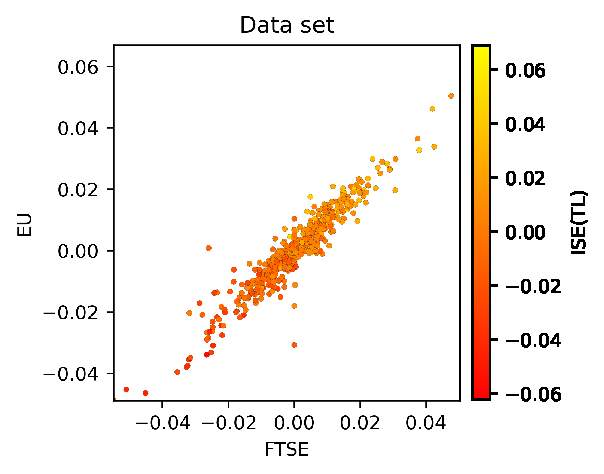
\includegraphics[width=\fourinarow]{figures/data.pdf}\label{fig:data}
		}
		\subfloat[\tiny LR.]{
			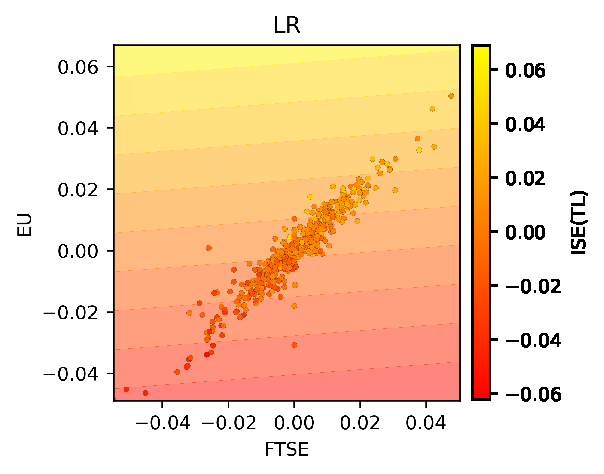
\includegraphics[width=\fourinarow]{figures/LR/model.pdf}\label{fig:lr}
		}
		\subfloat[\tiny \cart{} 6 leaves.]{
			\includegraphics[width=\fourinarow]{figures/LR/cart6.pdf}\label{fig:cart6}
		}
		\subfloat[\tiny \cart{} 10 leaves.]{
			\includegraphics[width=\fourinarow]{figures/LR/cart10.pdf}\label{fig:cart10}
		}
		\\
		\subfloat[\tiny \creepy{} constant out.]{
			\includegraphics[width=\fourinarow]{figures/LR/creepyK.pdf}\label{fig:creepyK}
		}
		\subfloat[\tiny \creepy{}.]{
			\includegraphics[width=\fourinarow]{figures/LR/creepy.pdf}\label{fig:creepy}
		}
		\subfloat[\tiny \gridex{}.]{
			\includegraphics[width=\fourinarow]{figures/LR/gridex.pdf}\label{fig:gridex}
		}
		\subfloat[\tiny \gridrex{}.]{
			\includegraphics[width=\fourinarow]{figures/LR/gridrex.pdf}\label{fig:gridrex}
		}
	\end{figure}

	\framebreak
	
	\begin{table}[]\centering
		\tiny
		\begin{tabular}{cccccc}
			\toprule
			Name & Type & Parameters & Rules & MAE data (BB) & R$^2$ data (BB) \\
			\midrule
			\midrule
			\cart6 & \cart{} & Max leaves = 6 & 6 & 0.01 (0.00) & 0.42 (0.78) \\
			& & Max depth = Unbounded & & & \\
			\midrule
			\cart10 & \cart{} & Max leaves = 10 & 10 & 0.01 (0.00) & 0.43 (0.85) \\
			& & Max depth = Unbounded & & & \\
			\midrule
			\creepy-K & \creepy{} & Max depth = 6 & 7 & 0.01 (0.01) & 0.10 (0.16) \\
			& & Threshold = 0.001 & & & \\
			& & Output = constant & & & \\
			\midrule
			\creepy-L & \creepy{} & Max depth = 6 & 2 & 0.01 (0.00) & 0.44 (0.93) \\
			& & Threshold = 0.001 & & & \\
			& & Output = linear combination & & & \\
			\midrule
			\gridex{} & \gridex{} & Max depth = 2 & 7 & 0.01 (0.01) & 0.30 (0.61) \\
			& & Threshold = 0.01 & & & \\
			& & Splits = 3 if feature importance $>$ 0.8 else 1 & & & \\
			\midrule
			\gridrex{} & \gridrex{} & Max depth = 2 & 1 & 0.01 (0.00) & 0.44 (1.00) \\
			& & Threshold = 0.1 & & & \\
			& & Splits = 2 & & & \\
			\bottomrule
		\end{tabular}
	\end{table}

	\framebreak
	
	\begin{table}[]\centering
		\scriptsize
		\begin{tabular}{ccccc}
			\toprule
			Name & Predictive loss & Readability loss & Coverage loss & Quality score \\
			\midrule
			\cart6 & 0.58 & 6 & 1.00 & 3.48 \\
			\cart10 & 0.57 & 10 & 1.00 & 5.70 \\
			\creepy-K & 0.90 & 7 & 1.00 & 6.30 \\
			\creepy-L & 0.56 & 2 & 1.00 & 1.12 \\
			\gridex{} & 0.70 & 7 & 1.01 & 4.95 \\
			\gridrex{} & 0.56 & 1 & 1.01 & 0.57 \\
			\bottomrule
		\end{tabular}
	\end{table}
	
	\begin{figure}[]\centering
		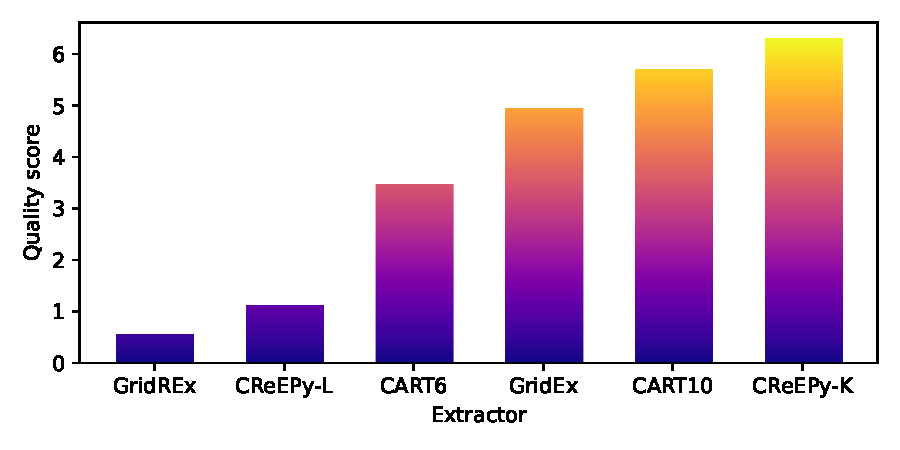
\includegraphics[width=.675\linewidth]{figures/bcr.pdf}
	\end{figure}

	\framebreak
	
	Rules extracted with \cart{} (6 leaves):
	\begin{lstlisting}
ise(BOVESPA, DAX, EM, EU, FTSE, NIKKEI, SP, -0.02) :-
		EU =< -0.00, EU =< -0.02.
ise(BOVESPA, DAX, EM, EU, FTSE, NIKKEI, SP, 0.00) :-
		EU =< -0.00, EU > -0.02.
ise(BOVESPA, DAX, EM, EU, FTSE, NIKKEI, SP, 0.00) :-
		EU > -0.00, EU =< 0.01, EM =< 0.00.
ise(BOVESPA, DAX, EM, EU, FTSE, NIKKEI, SP, 0.00) :-
		EU > -0.00, EU =< 0.01, EM > 0.00.
ise(BOVESPA, DAX, EM, EU, FTSE, NIKKEI, SP, 0.01) :-
		EU > -0.00, EU > 0.01, EM =< 0.01.
ise(BOVESPA, DAX, EM, EU, FTSE, NIKKEI, SP, 0.02) :-
		EU > -0.00, EU > 0.01, EM > 0.01.
	\end{lstlisting}

	\framebreak
	
	Equivalent rules (\cart{}6):
	\begin{lstlisting}
ise(BOVESPA, DAX, EM, EU, FTSE, NIKKEI, SP, -0.02) :-
		EU =< -0.02.
ise(BOVESPA, DAX, EM, EU, FTSE, NIKKEI, SP, 0.00) :-
		EU =< -0.00.
ise(BOVESPA, DAX, EM, EU, FTSE, NIKKEI, SP, 0.00) :-
		EU =< 0.01, EM =< 0.00.
ise(BOVESPA, DAX, EM, EU, FTSE, NIKKEI, SP, 0.00) :-
		EU =< 0.01.
ise(BOVESPA, DAX, EM, EU, FTSE, NIKKEI, SP, 0.01) :-
		EM =< 0.01.
ise(BOVESPA, DAX, EM, EU, FTSE, NIKKEI, SP, 0.02).
	\end{lstlisting}

	\framebreak
	
	Rules extracted with \creepy{} (linear outputs):
	\begin{lstlisting}
ise(BOVESPA, DAX, EM, EU, FTSE, NIKKEI, SP, ISE) :-
		FTSE in [-0.05, 0.04], EU in [-0.04, 0.04],
		ISE is -0.02 BOVESPA - 0.05 DAX - 0.05 EM + 0.63 NIKKEI + 0.47 SP.
ise(BOVESPA, DAX, EM, EU, FTSE, NIKKEI, SP, ISE) :- 
		ISE is 0.01.
	\end{lstlisting}

\end{frame}

\section{Conclusions}

\begin{frame}[c]{Conclusions}
	\vfill
	\begin{block}{In this paper}
		\smallskip
		\begin{itemize}
			\item we focus on the need of metrics assessing knowledge quality for SKE
			\begin{itemize}
				\item based on readability, predictive performance and completeness
			\end{itemize}
			\smallskip
			\item we observe that knowledge readability cannot be trivially assessed
			\begin{itemize}
				\item it can be done at a macrolevel, as a whole
				\item it cannot be done at a microlevel, for individual rules
			\end{itemize}
			\smallskip
			\item we recognise that a human interaction is required 
			\smallskip
			\item we propose a metric to assess the knowledge quality
			\begin{itemize}
				\item encompassing readability, predictive performance and completeness
			\end{itemize}
		\end{itemize}	
		\smallskip
	\end{block}

	\vfill
\end{frame}

\begin{frame}[c]{Future Works}
	\vfill
	\begin{block}{Future Works}
		\medskip
		\begin{itemize}
			\item Enhance the proposed metric for the knowledge quality
			\medskip
			\item Consider the readability microlevel
			\medskip
			\item Consider the human interaction
			\medskip
			\item Exploit the metric for autoML tasks
		\end{itemize}
		\medskip
	\end{block}
	\vfill
\end{frame}

%===============================================================================
\section*{}
%===============================================================================

%/////////
\frame{\titlepage}
%/////////

\section*{\refname}

\setbeamertemplate{page number in head/foot}{}
\begin{frame}[t,allowframebreaks,noframenumbering]{\refname}
	\scriptsize
	\bibliographystyle{apalike}
	\bibliography{SC-AITA-2023}
\end{frame}

\end{document}